\begin{figure}[htbp]
\centering
\begin{tikzpicture}[causal,x=1cm,y=1cm,
 ch05amino/.style={circle,draw,fill=orange!35!red!25,minimum size=5.8mm,inner sep=1pt,font=\scriptsize},
 ch05bio/.style={font=\scriptsize,align=center}]
% 翻译原图的肽合成示意；核苷酸和氨基酸缩写按原图保留。
\begin{scope}[x=.82cm,y=.82cm]
\path[draw,fill=olive!50!gray]
 (2.1,1.6) .. controls (2.7,1.8) and (2.6,3.2) .. (3.8,3.2)
 .. controls (5.2,3.1) and (5.4,2.3) .. (5.3,1.2)
 .. controls (5.15,.1) and (4.4,.25) .. (2.9,.4)
 .. controls (2.4,.45) and (3.6,1.1) .. (2.1,1.6)--cycle;
\node[ch05bio] at (4.15,.86){核糖体};
\filldraw[fill=gray!50!green!15,draw=gray!80] (0,1.45) rectangle (8,1.72);
\foreach \x in {.08,.33,...,7.85}{
 \filldraw[fill=gray!50!green!15,draw=gray!80] (\x,1.72) rectangle ++(.1,.18);}
\node[font=\scriptsize,inner sep=1pt,fill=gray!50!green!15] at (3.5,1.58){U G G A A A G A U U U C};
\node[ch05bio] at (6.8,1.04){信使 RNA};
\foreach \x/\triplet in {3.15/U U U,4.1/C U A}{
 \path[draw,fill=yellow!85] (\x-.36,1.9)--(\x-.36,3.35)--(\x+.36,3.35)
 --(\x+.36,1.9)--(\x+.2,1.9)--(\x+.16,2.12)--(\x+.05,2.12)
 --(\x+.01,1.9)--(\x-.1,1.9)--(\x-.14,2.12)--(\x-.25,2.12)--(\x-.29,1.9)--cycle;
 \node[ch05bio,font=\tiny] at (\x,2.85){tRNA};
 \node[ch05bio,font=\tiny] at (\x,2.22){\triplet};
 \draw[thick] (\x,3.35)--(\x,4.1);}
\node[ch05amino] (ch05lys) at (3.15,4.1){Lys};
\node[ch05amino] (ch05asp) at (4.1,4.1){Asp};
\node[ch05amino] (ch05trp) at (2.25,4.38){Trp};
\node[ch05amino] (ch05aa2) at (1.57,4.95){};
\node[ch05amino] (ch05aa1) at (.93,5.51){};
\draw (ch05aa1)--(ch05aa2)--(ch05trp)--(ch05lys)--(ch05asp);
\node[ch05bio,anchor=west] at (1.8,5.55){正在延长的肽链};
\begin{scope}[shift={(1.1,3.55)},rotate=20]
\draw[thick] (0,.65)--(0,1.1);
\path[draw,fill=yellow!85] (-.35,-.8)--(-.35,.65)--(.35,.65)--(.35,-.8)
 --(.21,-.8)--(.17,-.57)--(.06,-.57)--(.02,-.8)--(-.09,-.8)--(-.13,-.57)--(-.24,-.57)--(-.28,-.8)--cycle;
\node[ch05bio,rotate=20] at (0,.05){tRNA};
\node[ch05bio,rotate=20] at (0,-.48){A C C};
\end{scope}
\node[ch05bio,anchor=east] at (.72,3.14){离开的\\空载 tRNA};
\draw[ed,very thick] (2.2,2.35)--(1.62,2.77);
\begin{scope}[shift={(6.3,3.48)},rotate=20]
\draw[thick] (0,.65)--(0,1.23);
\node[ch05amino] at (0,1.5){Phe};
\path[draw,fill=yellow!85] (-.35,-.8)--(-.35,.65)--(.35,.65)--(.35,-.8)
 --(.21,-.8)--(.17,-.57)--(.06,-.57)--(.02,-.8)--(-.09,-.8)--(-.13,-.57)--(-.24,-.57)--(-.28,-.8)--cycle;
\node[ch05bio,rotate=20] at (0,.05){tRNA};
\node[ch05bio,rotate=20] at (0,-.48){A A G};
\end{scope}
\node[ch05bio,anchor=west] at (6.65,4.13){进入的、结合\\氨基酸的 tRNA};
\draw[ed,very thick] (5.9,2.94)--(5.13,1.96);
\node[font=\small] at (4,-.05){肽合成};
\end{scope}
% 上：因果方向；下：反因果方向。绿色为预测，红色为因果关系。
\node[vtx] (ch05ax) at (8.6,2.8){$X$};
\node[vtx] (ch05ay) at (11.6,2.8){$Y$};
\node (ch05anx) at (8.6,1.3){$N_X$};
\node (ch05any) at (11.6,1.3){$N_Y$};
\draw[ed,red!85!black] (ch05ax)--node[below]{$\varphi$}(ch05ay);
\draw[ed,green!60!black,bend left=27] (ch05ax) to (ch05ay);
\draw[ed,blue!70!black] (ch05anx)--node[right]{$\mathrm{id}$}(ch05ax);
\draw[ed,red!85!black] (ch05any)--(ch05ay);
\node[inner sep=0pt] at (1.05,-1.7){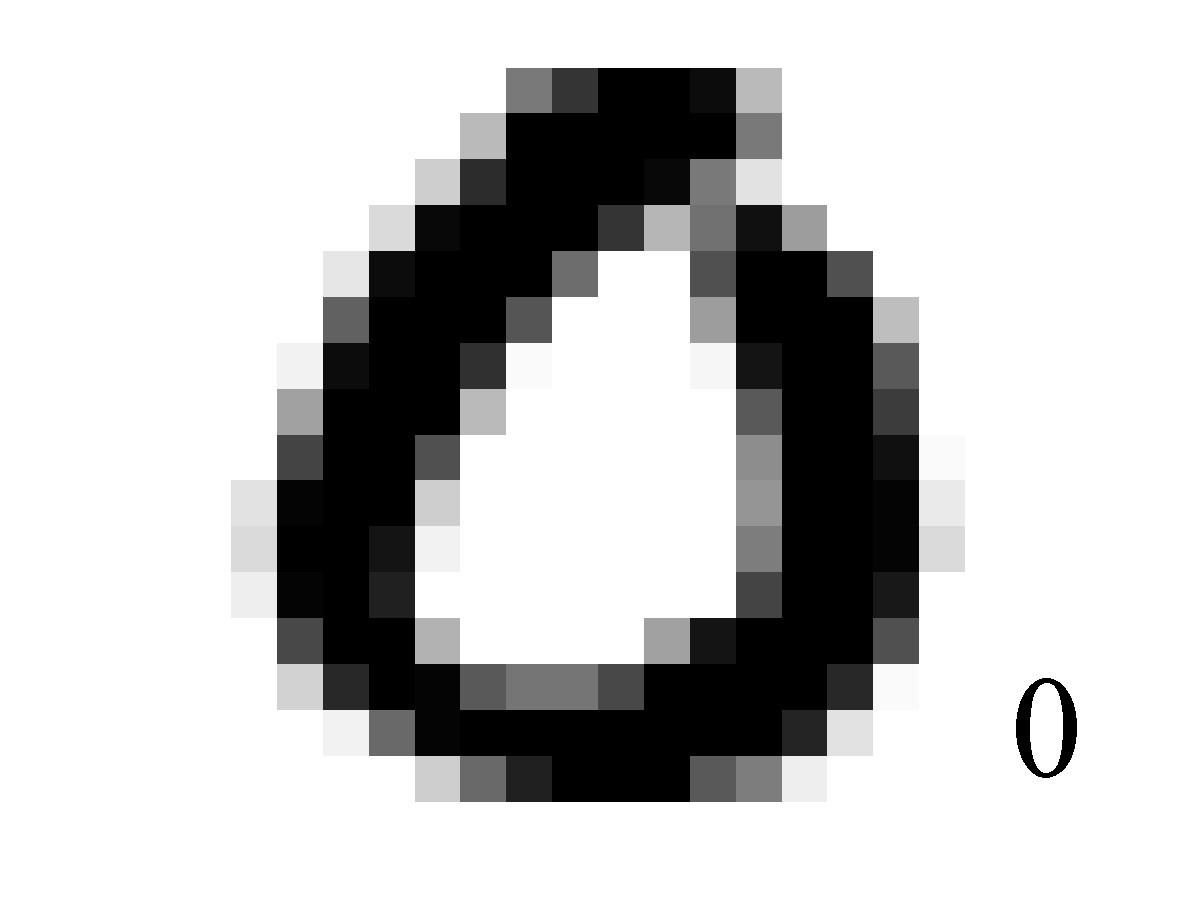
\includegraphics[width=2cm]{data/ch05_digit_0.jpg}};
\node[inner sep=0pt] at (3.35,-1.7){
\includegraphics[width=2cm]{data/ch05_digit_2.jpg}};
\node[inner sep=0pt] at (5.65,-1.7){
\includegraphics[width=2cm]{data/ch05_digit_7.jpg}};
\node[vtx] (ch05bx) at (8.6,-1.7){$X$};
\node[vtx] (ch05by) at (11.6,-1.7){$Y$};
\node (ch05bnx) at (8.6,-3.2){$N_X$};
\node (ch05bny) at (11.6,-3.2){$N_Y$};
\draw[ed,red!85!black] (ch05by)--node[below]{$\varphi$}(ch05bx);
\draw[ed,green!60!black,bend left=27] (ch05bx) to (ch05by);
\draw[ed,red!85!black] (ch05bnx)--(ch05bx);
\draw[ed,blue!70!black] (ch05bny)--node[right]{$\mathrm{id}$}(ch05by);
\end{tikzpicture}
\caption[因果与反因果预测任务]{上：称为核糖体的复杂机制 $\varphi$ 将 mRNA 信息 $X$ 翻译为蛋白质链 $Y$。\protect\footnotemark 根据 mRNA 预测蛋白质，是沿因果方向展开的学习问题；此时，预测方向（绿色箭头）与因果作用方向（红色箭头）一致。下：在手写数字识别中，我们试图根据书写者生成的图像 $X$，推断类别标签 $Y$，即书写者的意图。这是一个沿反因果方向展开的问题。}
\label{fig:ch05-learning-directions}
\end{figure}
\footnotetext{原肽合成图由用户“Boumphreyfr”提供：\url{https://commons.wikimedia.org/wiki/File:Peptide_syn.png}。许可为 CC BY-SA 3.0（\url{http://creativecommons.org/licenses/by-sa/3.0}）或 GFDL（\url{http://www.gnu.org/copyleft/fdl.html}）。本译稿以 TikZ 重绘其示意结构并翻译图中文字。}
